% lint-skip: 未完成ステータス（figure/table caption 未対応，人手チェック時に解消予定）
\documentclass[../../main.tex]{subfiles}
\begin{document}

\begin{flushright}
  \footnotesize\textit{【自動文字起こし・要確認】}
\end{flushright}

{\bf [解答]}
\begin{figure}[htbp]
  \centering
  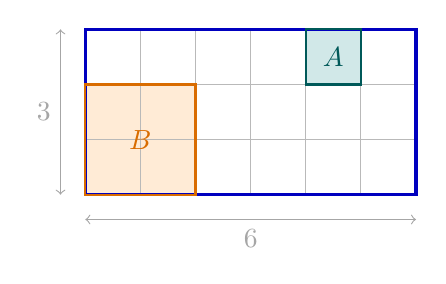
\begin{tikzpicture}[scale=0.7]
    \fill[orange!16] (0,0) rectangle (2,2);
    \fill[teal!18] (4,2) rectangle (5,3);
    \draw[gray!55,thin,step=1] (0,0) grid (6,3);
    \draw[blue!75!black,very thick] (0,0) rectangle (6,3);
    \draw[orange!85!black,thick] (0,0) rectangle (2,2);
    \draw[teal!70!black,thick] (4,2) rectangle (5,3);
    \node[orange!85!black] at (1,1) {$B$};
    \node[teal!70!black] at (4.5,2.5) {$A$};
    \draw[<->,gray!70] (0,-0.45)--(6,-0.45) node[midway,below] {$6$};
    \draw[<->,gray!70] (-0.45,0)--(-0.45,3) node[midway,left] {$3$};
  \end{tikzpicture}
  \caption{$6\times3$ の長方形と一辺1のタイル $A$、一辺2のタイル $B$}
\end{figure}
一辺1の正方形タイルをA

一辺2の正方形タイルをB

と名付ける．A, Bの用いた枚数

$a, b$ とすると（$a, b \in \mathbb{Z}_{\ge 0}$），面積から
\[ a + 4b = 18 \]
が必要で，
\[ (a, b) = (2, 4), (6, 3), (10, 2), (14, 1), (18, 0) \]
のいずれかである．又，長方形の形から，$b \le 3$ も必要であるから，$(a,b)=(2,4)$ は不適である．逆に，他の時は長方形をうまくうめることができて十分．

（試行回数$n$）$=a+b$に注意して，求める確率を$a_n$とおくと
\begin{align}
  a_9 &= {}_9\mathrm{C}_3 \cdot p^6 q^3 = 84 p^6 q^3 \\
  a_{12} &= {}_{12}\mathrm{C}_2 \cdot p^{10} q^2 = 66 p^{10} q^2 \\
  a_{15} &= {}_{15}\mathrm{C}_1 \cdot p^{14} q = 15 p^{14} q \\
  a_{18} &= p^{18} \\
  \text{otherwise} &\quad a_n = 0 \quad //
\end{align}

\end{document}
